\documentclass[a4paper]{article}

\usepackage[a4paper, total={7in, 10in}]{geometry}
\usepackage[T1,T2A]{fontenc}
\usepackage[utf8]{inputenc}
\usepackage[english,russian]{babel}
\usepackage{graphicx}
\graphicspath{ {./images/} }

\begin{document}

\title{\textit{\textbf{Лабораторная работа №401}}}
\author{Губанов Пётр, С01-019}
\maketitle

\clearpage

\title{\large{\textit{5. Задания к выполнению.}}}\\\\

\textbf{\textit{\underline{5.1.}}} Создать модуль и символ двоичного суммирующего счетчика (VCB4RE). Провести моделирование его работы. Начертить в тетради эскизы содержательных фрагменто полученных временных диаграмм.
\begin{center}
	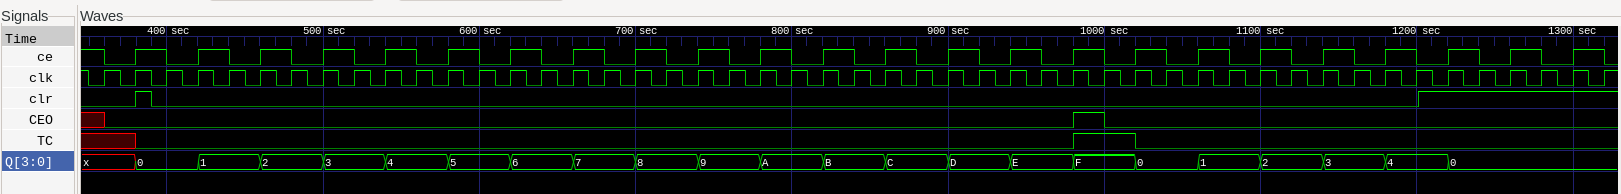
\includegraphics[scale=0.3]{../images/VCB4RE.png}
\end{center}

\textbf{\textit{\underline{5.2.}}} Создать модуль и символ декадного счетчика (VCD4RE). Провести моделирование его работы. Начертить в тетради эскизы содержательных фрагментов полученных временных диаграмм.
\begin{center}
	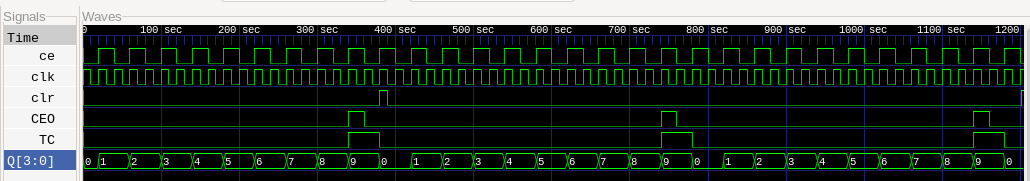
\includegraphics[scale=0.45]{../images/VCD4RE.png}
\end{center}

\textbf{\textit{\underline{5.3.}}} Создать модуль и символ двоичного вычитающего счетчика (VCBDmSE). Провести моделирование его работы. Начертить в тетради эскизы содержательных фрагментов полученных временных диаграмм.
\begin{center}
	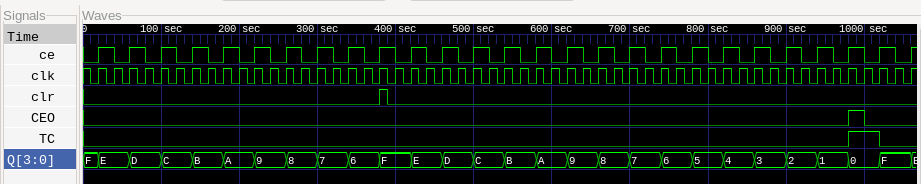
\includegraphics[scale=0.5]{../images/VCBDmSE.png}
\end{center}

\textbf{\textit{\underline{5.4.}}} Создать модуль и символ реверсивного счетчика (VCBmCLED). Провести моделирование его работы. Начертить в тетради эскизы содержательных фрагментов полученных временных диаграмм.
\begin{center}
	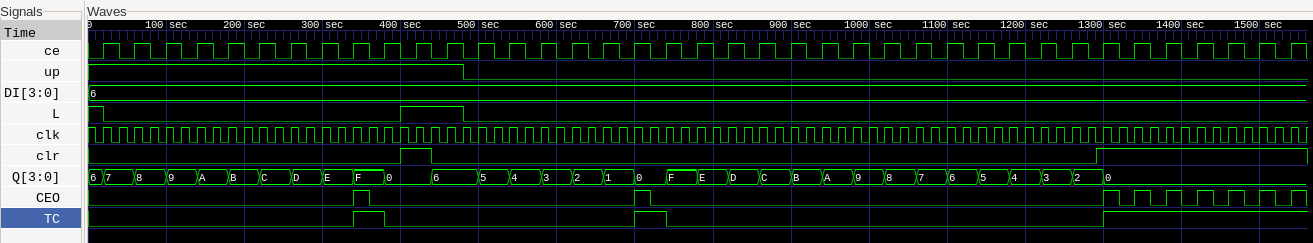
\includegraphics[scale=0.39]{../images/VCBmCLED.png}
\end{center}

\textbf{\textit{\underline{5.5.}}} Создать модуль и символ счетчика Джонсона (VCJ4RE). Провести моделирование его работы. Начертить в тетради эскизы содержательных фрагментов полученных временных диаграмм.
\begin{center}
	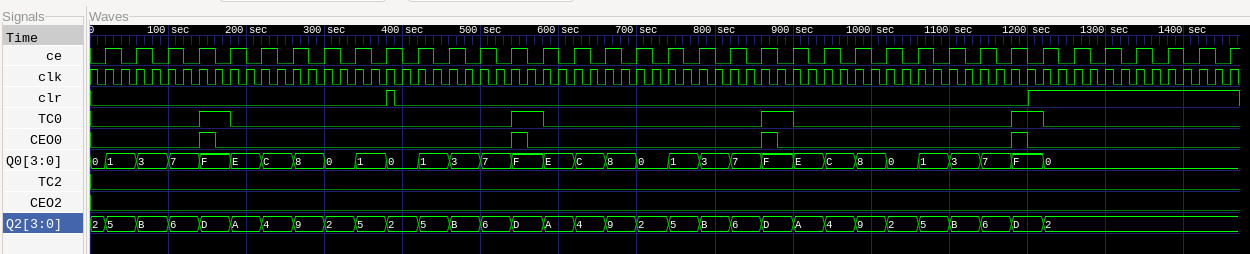
\includegraphics[scale=0.4]{../images/VCJ4RE.png}
\end{center}

\textbf{\textit{\underline{5.6.}}} Создать модуль и символ счетчика в коде Грея (VCGrey4RE). Провести моделирование его работы. Начертить в тетради эскизы содержательных фрагментов полученных временных диаграмм.
\begin{center}
	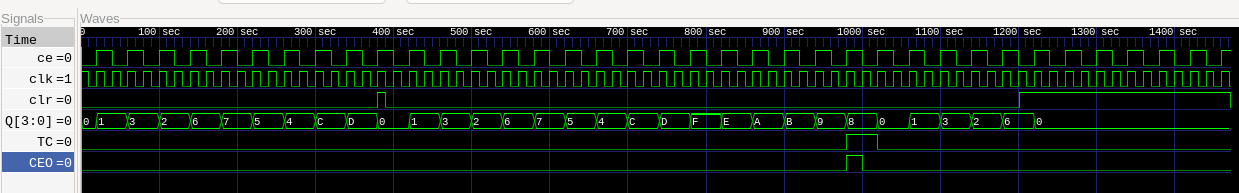
\includegraphics[scale=0.4]{../images/VCGrey4RE.png}
\end{center}

\textbf{\textit{\underline{5.7.}}} Создать модуль генератора последовательного включения цифр семи сегментного индикатора (Gen4an), мультиплексора 4-х битных цифр (MUX16\_4), генератора сигналов разрешения счета (Gen1ms), генератора точки (Gen\_P), дешифратора для семи сегментного индикатора (D7seg). Необходимо дополнить дешифратор индикацией HEX цифр: A, b, C, d, E, F. Создать модуль и символ DISPLAY индикатора.\\

\textbf{\textit{\underline{5.8.}}} Создать модуль и символ Gen\_Nms\_1s (см. в разделе Приложение) в соответствии с Вашим вариантом задания (N = 18). Этот генератор должен давать на выходе периодическую последовательность импульсов с длительностью Tclk (20 ns) и с периодом 1s - при низком уровне сигнала на входе mod (Tmod=0), и с периодом N*1ms - при высоком уровне сигнала на входе mod (Tmod=1).\\

\textbf{\textit{\underline{5.9.}}} Из составленных модулей составить схему (Sch1\_lab401) заданного варианта последовательности соединения счетчиков (вариант №4) с отображением их состояния на семисегментном индикаторе.\\

\begin{center}
	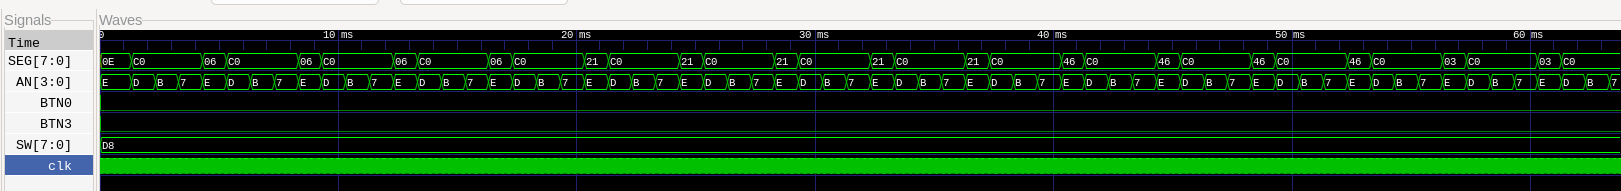
\includegraphics[scale=0.3]{../images/my_counter.png}
\end{center}

\textbf{\textit{\underline{5.10.}}} Провести имплементацию, создать загрузочный файл конфигурации для данной схемы Sch1\_lab401.bit (Generate Programming File) для загрузки в ПЛИС или *.mcs (Configure Target Device) для загрузки в ПЗУ (XCF04S).\\

\title{\large{\textit{6. Задания к сдаче.}}} \\\\

\textbf{\textit{\underline{6.1.}}} Создать модуль подавления дребезга кнопки BTN2, обеспечивающий изменение состояния счетчиков на 1 от каждого нажатия кнопки. Соединить в схеме рис.4.1 входы CE используемых счетчиков параллельно и соединить с выходом модуля подавления кнопки. Продемонстрировать работу устройства на макете.\\

\textbf{\textit{\underline{6.2.}}} Создать модуль измерения периода сигнала на выходе CEO генератора Gen\_Nms\_1s. Модуль должен обеспечить отображение на семи сегментном индикаторе макета период сигнала на выходе CEO генератора Gen\_Nms\_1s в десятичном виде. Отладить работу модуля и продемонстрировать на макете при двух значениях SW[7].

\end{document}
